O comportamento parlamentar envolve uma série de ações sociais. Podemos dividi-las em três tipos \cite{behm_sheep_2019}: (\textit{i}) legislativas, que focam na formulação de políticas e na busca de construção de maiorias favoráveis a determinada iniciativa política; (\textit{ii}) atividades de fiscalização, que estão ligadas à capacidade de os parlamentares obterem informações e fiscalizarem demais órgãos; e (\textit{iii}) atividades de publicidade, que objetivam comunicar aos seus eleitores seus posicionamentos. 

A literatura sobre o comportamento parlamentar é ampla e focaliza em diferentes aspectos do comportamento parlamentar. Uma ampla gama de atividades recebem atenção da literatura, tais como autoria de proposições legislativas \cite{crisp2007incentives, gagliarducci2011electoral}, emendas orçamentárias \cite{kerevel2015pork}, discursos em plenária  \cite{proksch2012institutional}, questionamentos parlamentares \cite{fernandes2019impact, russo2021mps}, participação em determinadas comissões  \cite{crisp2007incentives,stratmann2002plurality}, troca de partido político \cite{klein2018personal}, dissenso em votações  \cite{carey2007competing, sieberer2010behavioral}, entre outros.

A literatura sobre comportamento parlamentar é amplamente influenciada pela abordagem racionalista, que compreende as ações dos parlamentares como um cálculo racional para maximizar seus próprios interesses, especialmente as chances de reeleição \cite{mayhew2004congress}. Essa abordagem, embora dominante, não é a única, e outros incentivos também desempenham um papel importante na motivação dos parlamentares.

É importante ressaltar que maximizar as chances de reeleição não é sinônimo de maximizar a quantidade de votos, mas sim de obter o número suficiente para garantir a reeleição \cite{mayhew2004congress}. Nesse sentido, os parlamentares tendem a ser ativos no parlamento, sinalizando aos eleitores seu trabalho em prol destes e, consequentemente, aumentando suas chances de reeleição.

Parte da literatura, porém, ressalta que tais incentivos somente existem em determinadas configurações institucionais, particularmente em sistemas eleitorais personalistas \cite{aleman2009comparing, kessler1996dynamics, krehbiel1995cosponsors} ou com forte voto de preferência \cite{brauninger2012personal}.

Mesmo na ausência desses mecanismos, a atividade parlamentar não cessa. Outros incentivos também são encontrados na literatura  \cite{strom1997rules}, tais como o de re-seleção e promoção \cite{martin2014electoral, rahat2001candidate,shomer2009candidate};  e instituições parlamentares, como partidos políticos e comitês legislativos, nas quais o parlamentar é socializado \cite{andeweg2011pathways, asher1973learning, louwerse_personalised_2016}.

Assim, os parlamentares podem objetivar tanto maximizar a chance de reeleição (\textit{vote-seeking}, quanto a re-seleção, ou renomeação, progressão na carreira política (\textit{carrer-seeking}) por meio de nomeação a cargos partidários - liderança partidária - ou legislativos - lideranças interpartidárias - \cite{strom1997rules} e elaboração de políticas (\textit{policy-seeking}) \cite{muller1999}

As atividades parlamentares voltadas para a busca por votos, ou \textit{vote-seeking}, são aquelas que visam aumentar a visibilidade e a popularidade do parlamentar junto ao eleitorado. Mayhew (\citeyear{mayhew2004congress}) propôs uma tipologia dessas atividades dos congressistas norte-americanos, classificando-as em três categorias: (\textit{i}) propaganda, (\textit{ii})posicionamento político e (\textit{iii}) reivindicação de crédito. 

As duas primeiras categorias, propaganda e posicionamento político, visam aumentar a visibilidade e a imagem positiva do congressista perante seu eleitorado, sem a necessidade de realizações políticas concretas. Em contrapartida, a reivindicação de crédito exige que o parlamentar participe ativamente da produção de resultados políticos desejáveis para seus eleitores e que consiga se apresentar como o responsável por tais resultados, o que é desafiador em um Congresso com muitos membros. Para superar esse desafio, a distribuição de benefícios particularizados permite que o parlamentar vincule seu nome a uma medida de forma crível, incentivando-o a buscar a aprovação de legislação ou outros resultados políticos que beneficiem seu distrito ou grupos específicos nele localizados.

Esses incentivos eleitorais são fortemente dependentes do sistema eleitoral. Diferentes sistemas eleitorais produzem diferentes incentivos e restrições para os parlamentares, moldando suas estratégias de busca por votos e suas prioridades políticas. 

Samuels (\citeyear{samuels1997determinantes}) argumenta que os sistema de voto único não-transferível, de voto único transferível e de representação proporcional de lista aberta favorecem o voto pessoal.Nesses sistemas, a capacidade do parlamentar de construir uma base eleitoral pessoal é fundamental para sua reeleição. Em sistemas majoritários, por exemplo, parlamentares que estão mais vulneráveis eleitoralmente têm mais chance de apresentarem projetos \cite{bowler2010private}

Ibenskas \citeyear{Ibenskas2021} discute a reeleição dos \acrshor{mpe}s, enfatizando sua dependência dos eleitores de seus países de origem e dos partidos nacionais. O estudo sugere que os \acrshort{mpe}s, especialmente sob os sistemas de lista flexível, lista aberta ou voto único transferível, buscam se envolver com organizações que aumentam seu apelo eleitoral.

É importante diferenciar os efeitos do sistema eleitoral quanto à reeleição (explicado anteriormente) e quanto à seleção. Viganò (\citeyear{vigano2024electoral}) estudou os efeitos da reforma eleitoral italiana de 2005, que mudou de um sistema misto para um sistema proporcional, na atenção dos parlamentares reeleitos a questões locais. Os resultados mostram que os parlamentares anteriormente eleitos em distritos de membro único não diminuíram significativamente sua atenção a questões locais após a reforma, indicando que os incentivos eleitorais sozinhos não são suficientes para modificar o comportamento dos parlamentares, e que os efeitos de seleção devem ser também considerados.

Um outro aspecto que deve ser mencionado é que o o tamanho e a diversidade socioeconômica do eleitorado de determinado parlamentar também impacta seu comportamento legislativo. Willumsen, Stecker e Goetz (\citeyear{willumsen_electoral_2019}) encontraram evidências de que há uma relação positiva entre o tamanho do distrito e a quantidade de questões e de proposições de senadores australianos. A diversidade do eleitorado, entretanto, está negativamente relacionada com a atividade legislativa \cite{willumsen_electoral_2019}.

Além dos incentivos eleitorais e institucionais, outros fatores também influenciam o comportamento parlamentar individual. A participação em comitês legislativos, a formação profissional, o partido político e o lobby são alguns dos fatores que podem moldar as ações dos parlamentares. Tais fatores estão relacionados com os objetivos de progressão na carreira (\textit{carreer-seeking}) e formulação de políticas (\textit{policy-seeking}).

O trabalho do parlamentar em comissões está correlacionado com esses dois objetivos \cite{daniel2015career}. A presença em comissões fomenta a possibilidade de formulação de políticas. O sucesso na realização de objetivos políticos leva a novas funções e cargos de poder, de modo que ambos os objetivos estão relacionados \cite{daniel2015career}. 

A expertise, experiência e lealdade partidária são fatores importantes que impactam na capacidade de o parlamentar não só participar em comissões, mas também concretizar seus objetivos de carreira e de políticas públicas \cite{chiru2020loyal}

A presença em comissões também é um indiciativo da agenda legislativa do parlamentar. Como as comissões normalmente se organizam em torno de temas, os parlamentares podem buscar participar daquelas cujos temas estão correlacionados aos seus objetivos políticos \cite{schiller1995senators}.

Um indicativo importante desses objetivos políticos do parlamentar está ligado ao seu \textit{background} ocupacional \cite{damgaard1980dilemma}. Não só sua ocupação prévia está relacionada com a suas áreas de interesses e expertise, mas também com a sua auto-seleção para comissões \cite{hamm2011committee, mcelroy2006committee, yordanova2009rationale} e com o foco da sua agenda legislativa \cite{burden2015personal}.

O partido político ao qual o parlamentar pertence também é um fator determinante de seu comportamento. A ideologia partidária, a disciplina partidária e a posição do partido no governo influenciam as posições dos parlamentares em relação a diferentes temas, suas alianças políticas e suas estratégias legislativas. Um comportamento que vá de encontro ao estabelecido pelo partido pode ser sancionado com diferentes mecanismos, tais como pelo controle de seleção de candidatos que vão concorrer a alguma eleição \cite{carey2007competing, hix2004electoral} e recompensas e sanções da liderança \cite{bressanelli2016impact}.

No contexto do \acrlong{pe}, vale destacar, não há regras específicas que formalizem a obrigação de os parlamentares seguirem os seus partido. Contudo, as lideranças partidárias mesmo assim tendem a sancionar comportamentos contrários à direção partidária por meio dos mecanismos mencionados acima \cite{carey2007competing, hix2004electoral, bressanelli2016impact}.

Outro aspecto relacionado aos partidos que afetam o comportamento parlamentar que deve ser mencionado é a ideologia partidária. Entendida como um conjunto de regras institucionais informais \cite{helmke2012informal}, a ideologia partidária pode ser compreendida como um conjunto de regras e valores que guiam o comportamento parlamentar \cite{hix2004electoral}. Parlamentares de partidos considerados como verdes, alternativos e libertários tendem a publicizar mais seus contatos com grupos de interesse, por exemplo, quando comparados a parlamentares de partidos tradicionalistas, autoritários e nacionalistas \cite{font_legislative_2023}.

O status do partido no governo também é um fator que deve ser levado em conta ao se estudar o comportamento parlamentar. Os partidos podem ser tornar \textit{veto players}, influenciando sua capacidade de negociar com o governo \cite{tsebelis2002veto}. Assim, o potencial de políticas que modifiquem o \textit{status quo} é menor quando partidos da oposição fazem parte do processo de tomada de decisão \cite{ganghof2006government}. 

Com base na revisão da literatura apresentada, podemos identificar pelo menos três componentes que afetam o comportamento parlamentar: (\textit{i}) o país do parlamentar; (\textit{ii}) o seu partido; e (\textit{iii}) aspectos individuais. A imagem abaixo traz uma representação gráfica desse \textit{framework} de análise do comportamento parlamentar:

    \begin{figure}[h]
        \caption{\textit{Framework} de análise do comportamento parlamentar}
        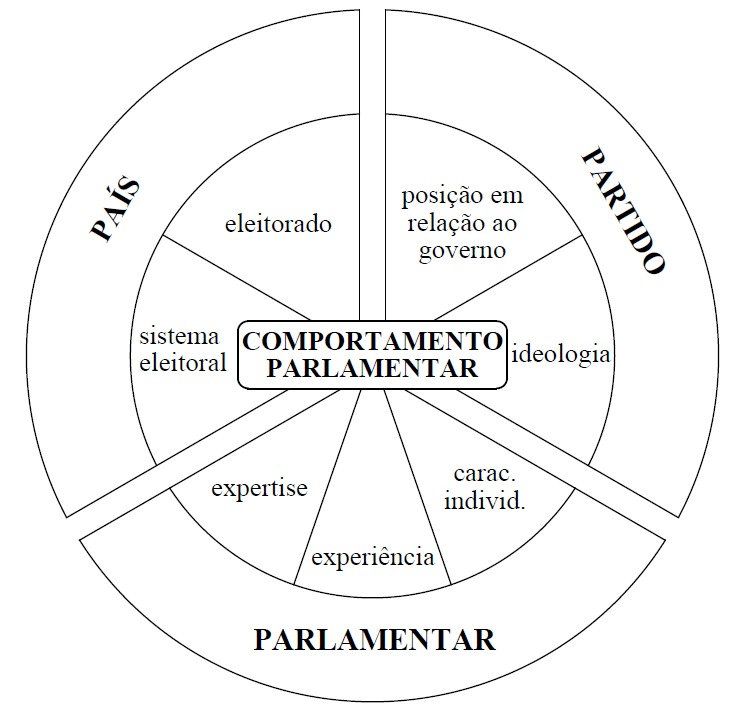
\includegraphics[width=\textwidth]{imgs/framework_compt_parlamentar.jpg}
        \label{fig:framework}
        \centering
        Fonte: o autor (2024).
    \end{figure}
    
    A componente do país do parlamentar envolve aspectos como o sistema eleitoral pelo qual é eleito e as características do eleitorado (tamanho do distrito e diversidade socio-econômica). Como visto no início desta seção, essa componente é extensivamente enfatizada pela literatura institucional \cite{mayhew2004congress}.
    
    O partido político ao qual pertence determinado parlamentar influencia o seu comportamento por meio da ideologia partidária, e da posição em relação ao governo. Partidos com maior disciplina e mais ideológicos podem estabelecer dinâmicas de comportamento. Além disso, a posição do partido no governo impacta a capacidade de um parlamentar influenciar na tomada de decisão.
    
    Os aspectos individuais do parlamentar podem ser sistematizados em: expertise, experiência e características individuais. Sua expertise, muito vinculada às ocupações prévias, influencia sua agenda legislativa de interesse. Além disso, a experiência política do parlamentar favorece o reconhecimento pelos pares e, assim, impacta seus objetivos políticos.

    Outras características individuais, como gênero, também podem influenciar o comportamento parlamentar. Hage e Ringe (\citeyear{hage2024works}), por exemplo, identificaram que parlamentares que compartilham características comuns (colaborações prévias em outros projetos, gênero e expertise) tendem a trabalhar mais em conjunto. 

    Com o \textit{framework}, busco destacar que o comportamento parlamentar é multifacetado e é o resultado dessas três dimensões. Não basta, portanto, olharmos apenas para o sistema eleitoral para entender os objetivos do parlamentar. Devemos incluir na análise tanto a dimensão partido, quando suas idiossincrasias. Mesmo, portanto, em sistemas centrados no candidato, que favorecem o voto pessoal, a expertise, a experiência e a situação do seu partido em relação ao governo,  por exemplo, também podem exercer efeitos sobre o comportamento parlamentar. Trata-se, portanto, de uma proposta que busca unir as diferentes escolas que estudam o fenômeno.
    

É nesse cenário complexo de interações simultâneas que os grupos de interesse buscam exercer influência. Os lobistas e grupos de interesse devem desenvolver estratégias e angariar recursos para tentar influenciar o comportamento parlamentar. Nesse sentido, buscam estabelecer relações de troca \cite{huwyler_no_2023} a fim de impactarem o comportamento do legislador. As evidências dessa relação causal, porém, é de difícil comprovação, envolvendo uma série de dificuldades metodológicas discutidas na seção \ref{section:effects}. O capítulo \ref{chapter:ue}, a seguir, resgata o contexto institucional da \acrshort{ue} com foco especial no \acrshort{pe}.
